\documentclass[]{article}



\usepackage{graphicx}
\usepackage{amsmath}
\usepackage{amsfonts}
\usepackage{amssymb}
\usepackage{lmodern}
\usepackage{pgfplots}
\usepackage{comment}
\usepackage{tikz}
\usetikzlibrary{datavisualization.formats.functions}
\usetikzlibrary{arrows}

\begin{document}
\title{Stochastik - Aufgabe 4}
\author{Tobias Reincke \\Matrikelnummer: 218203884}
\maketitle

\section{12 - Pareto-Verteilung}
\subsection{a}
$$
\int f(x) = -\frac{C}{\alpha x^\alpha} 
$$ $$
\int_{s}^{\infty} f(x) = \lim_{n \rightarrow \infty} -\frac{C}{\alpha n^\alpha} + \frac{C}{\alpha s^\alpha} = \frac{C}{\alpha s^\alpha}
$$
$$
\frac{C}{\alpha s^\alpha} = 1 \Leftrightarrow C = \alpha s^\alpha
$$

\subsection{b}
$$
\int_s^{\infty} f(x) = -\frac{\alpha s^\alpha}{\alpha x^\alpha} = -(\frac{s}{x}) ^\alpha 
$$

$$
\int_{s}^{x} f(x) dx = -(\frac{s}{x})^\alpha  +(\frac{s}{s}) ^\alpha = 1 -(\frac{s}{x})^\alpha
$$
$$
F(x) = \begin{cases} 
 \int_{-\infty}^{s} f(x) = 0  & x < s  \\
\int_{s}^{x} f(x) = 1 -(\frac{s}{x})^\alpha & x \geq s \\ 
\end{cases} 
$$

\subsection{c}
 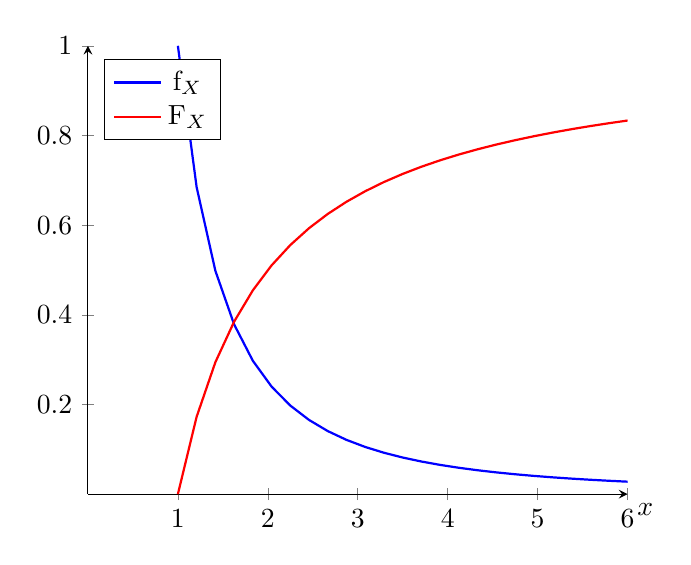
\begin{tikzpicture}

\begin{axis}[
legend pos=north west, 
axis x line=center,
axis y line=center,
xtick={ 1, 2,3 ,4, 5,6},
%xticklabels={ },
ytick={0,0.2 ,0.4,0.6,0.8, 1},
%yticklabels={, $ \frac{1}{b-a}$, 1},
%xticklabels={a,b},
xlabel={$x$},
ylabel={ },
xlabel style={below right},
ylabel style={above left},
xmin=0,
xmax=6,
ymin=0,
ymax=1]
\addplot [blue, mark=none,thick,domain=1:6] {1 /(x*x) };
\addlegendentry{$\text{f}_X$}
% \addplot [mark=none,domain=0:1] {y=1};
% \addplot [mark=none,domain=0:1] {y=4};
\addplot [red, mark=none, thick, domain=1:6] { 1 - 1/x };
\addlegendentry{$\text{F}_X$}
\end{axis}
%\draw[dashed] (1.72,0) -- (1.72,1.42);
%\draw[dashed] (6.88,0) -- (6.88,1.42);
\end{tikzpicture}

\subsection{d}
$$
	\mathbb{P} (0 \leq  X \leq 2) = \mathbb{P}(0 \leq X \leq  s=1 ) + \mathbb{P}( s=1 \leq X \leq 2)	= 0 + \int_{1}^{2} f(x) = - (\frac{1}{2})  + \frac{1}{1} = \frac{1}{2}
$$

$$ 
	\mathbb{P} (0 \leq  X \leq 2) = \mathbb{P}(0 \leq X \leq  s=1 ) + \mathbb( s=1 \leq X \leq 2)	= F(1) + F(2) = 0 +
	1 - \frac{1}{2} = \frac{1}{2}
$$

$$ \mathbb{P} (  5 \leq X \leq 8)  = \int_{5}^{8} f(x) = -\frac{1}{8} +  \frac{1}{5} = \frac{3}{40}  $$

$$ \mathbb{P} ( 5 \leq X \leq 8) = F(8) - F(5) = 1 - \frac{1}{8} - (1 - \frac{1}{5}) = \frac{1}{5} - \frac{1}{8} = \frac{3}{40} $$

Note: Bei der Dichtefunktion hätte man definitiv auch mit $ \int_0^8 f(x) dx - \int_2^5 f(x) dx $ die Wahrscheinlichtkeit berechnen k\"onnen 

\subsection{e}
$$
\frac{\alpha}{x} (\frac{s }{x}) ^ \alpha
$$
$$  f(x) ^4 = ( \frac{1}{x^2} )^4= \frac{1}{x^8} = \frac{1}{x^(1+7)} = \frac{7}{x}  (\frac{s}{x}) ^7    $$ 
$$  \rightarrow  s^7 = 1/7 \Leftrightarrow s = \sqrt[7]{\frac{1}{7}}   $$

Wenn $s = \sqrt[7]{\frac{1}{7}}$ dann muss
\begin{comment}

$$ \int_{\sqrt[7]{\frac{1}{7}}}^{\infty}  \frac{1}{x} (\frac{\sqrt[7]{\frac{1}{7}}{x}v }   dx =  -\frac{1}{\sqrt[7]{7x}} \] $$


\end{comment}
\section{Satz von Bayes}

Ich definiere folgende Ereignisse wie folgt:\\ 
A, eine 1 wird gesendet\\
B, eine 0 wird gesendet\\
C, eine 1 wird empfangen\\
D, eine 0 wird empfangen\\

$$ P(A) = \frac{7}{13}\ ,\ P(B) = \frac{6}{13}\ ,\ P(C) = P(A|C) *P(A) + P(B)* P(B|C)$$ $$P(D) = P(A)P(A|D) +P(B)P(B|D) $$ \\
$ P(A|D) = \frac{1}{5}\ ,\ \overline{P}(A|D) = P(A|C) \Rightarrow P(A| C) = \frac{4}{5} $\\
$P(B|C ) = \frac{1}{4},\  \overline{P}(B|C) = P(B|D) \Rightarrow P(B|D) = \frac{3}{4} $

Gefragt wird nach dem Ereigniss $P(C|A) $, d.h in Worten ausgedrückt, wie hoch ist die Wahrscheinlichkeit, dass eine 1 gesendet wurde, wenn eine 1 empfangen wurde.\\
Nach dem Satz von Bayes gilt:
$$ P(C|A) = \frac{P(A|C) *P(C)}{P(A)}$$

$$P(C) = \frac{7}{13} * \frac{4}{5}  +  \frac{6}{13} * \frac{1}{4}  = \frac{71}{650} $$
$$ P(C|A) = \frac{ \frac{4}{5} * \frac{71}{650}}{\frac{7}{13}} $$
Man dividiert 28/65 durch 7/13
$$P(C|A) = \frac{4 * 71 }{5 * 650 } = \frac{355}{3250} = 0.1092307692307 $$


\section{Wochentage}
\subsection{a)}
Wochentage sind Ereignisse:
A steht für Montag, 
B steht für Dienstag, 
C steht für Mittwoch,
D steht für Donnerstag,
E steht für Freitag
X steht f\"ur defekt.
$  \overline{X} $ steht dementsprechend f\"ur X ist korrekt.
Es gilt dementsprechend auch: $P(\overline{X}) = \overline{P(X)} $ 

$ P(A) = 0.15\
P(B) = 0.25\
P(C) = 0.2\
P(D) = 0.25\
P(E) = 0.15$

P(A | X) = 0.04
P(B | X) = 0.01
P(C | X) = 0.01
P(D | X) = 0.02
P(E | X) = 0.03

\subsection{b)}
$ P(X) = \sum_F P(F|X)   = P(A | X) +P(B | X) + P(C | X) + P(D | X) + P(E | X) = 0.11 $

\subsection{c)}
$P(X|A) = \frac{P(X) * P(A|X) }{P(A)} = \frac{0.11 * 0.04}{0.15}b = \frac{22}{750} $
\subsection{d)}
Da die Mengen D und E disjunkt sind, aka ein Ger\"at kann nicht freitags und donnerstags produziert worden sein, gilt:
$$ P( (D \cup E) | \overline{X} ) = \frac {P (\overline{X}| ( D \cup E)) * P(D \cup E) }{P(\overline{X})}  $$

$ P(\overline{X} | (D \cup E)) $ wird in e) berechnet. Daher werde ich einfach das Ergebniss nehmen. 
$ P(\overline{X}) = 0.89 $\\
$P (D \cup E) =  0.25 + 0.15 = 0.4$

$P( (D \cup E) | \overline{X} ) = \frac{0.02375 * 0.4}{0.89} = 0.0106741573033 $

\subsection{e)}

$$P (\overline{X} | D \cup E)  =\frac { P (\overline{X}) * P(D \cup E | \overline{X})  }{P(D \cup E)} =\frac{ \overline{P}(X) * (\frac{ P((D \cup E )\cap \overline{X})}{P(\overline{X})} )}{P(D \cup E)} $$


$$= \frac{ P( (D \cup E) \cap \overline{X})}{ P (D \cup E )}   ) = \frac{ P (D \cap \overline{X}) + P( E \cap \overline{X} ) }{ P  (D \cup E)} =\frac{  P(D) * P(X|D) + P(E) * P(X|E) }{P(D \cup E)}$$ $$ =\frac{0.25 * 0.02 + 0.15 * 0.03}{0.4} = 0.02375 $$
\end{document}
